%--------------------------------------------------------------
% thesis.tex 
%--------------------------------------------------------------
% Corso di Laurea in Informatica 
% - template for the main file of Informatica@Unifi Thesis 
% - based on Classic Thesis Style Copyright (C) 2008 
%   Andr\'e Miede http://www.miede.de   
%--------------------------------------------------------------
\documentclass[twoside,openright,titlepage,fleqn,
	headinclude,12pt,a4paper,BCOR=5mm,footinclude]{scrbook}

\usepackage[nottoc]{tocbibind}
%--------------------------------------------------------------
% Inputs for the title page 
%--------------------------------------------------------------
\newcommand{\myItalianTitle}{Titolo italiano\xspace}
\newcommand{\myEnglishTitle}{English title\xspace}
% use the right myDegree option
\newcommand{\myDegree}{Corso di Laurea in Informatica\xspace}
%\newcommand{\myDegree}{Corso di Laurea Magistrale in Informatica\xspace}
\newcommand{\myName}{Youness Aharram\xspace}
\newcommand{\mySupervisorTitle}{Relatore/Relatrice\xspace} %%% remove one of the two
\newcommand{\mySupervisorName}{\textit{prof. Daniele Baracchi}\xspace} 
\newcommand{\myCoSupervisorTitle}{Correlatore/Correlatrice\xspace} %%% optional: remove this command if the thesis has no Co-Supervisor
\newcommand{\myCoSupervisorName}{\textit{prof. Fabrizio Argenti}\xspace} %%% optional: remove this command if the thesis has no Co-Supervisor
\newcommand{\myTime}{Anno Accademico 2025-2026\xspace}
%--------------------------------------------------------------

\usepackage[utf8]{inputenc} 
\usepackage[T1]{fontenc} 

% switch italian and english, depending on the language of the thesis
% this will change the chapter titles
%\usepackage[italian]{babel}
\usepackage[english]{babel}
\usepackage{csquotes}

\usepackage[fleqn]{amsmath}  
\usepackage{ellipsis}
\usepackage{listings}
\usepackage{subfig}
\usepackage{caption}
\usepackage{appendix}
\usepackage{siunitx}
\usepackage[pdftex]{graphicx} 
\graphicspath{{./Figures/}}
 \usepackage[eulerchapternumbers,linedheaders,subfig,beramono,eulermath,
parts,dottedtoc]{classicthesis}

%--------------------------------------------------------------
% Layout setting
%--------------------------------------------------------------
\newlength{\abcd} 
\newcommand{\myfloatalign}{\centering} 
\setlength{\extrarowheight}{3pt} 
\captionsetup{format=hang,font=small}

\usepackage{geometry}
\geometry{
	a4paper,
	ignoremp,
	bindingoffset = 1cm, 
	textwidth     = 13.5cm,
	textheight    = 21.5cm,
	lmargin       = 3.5cm, 
	tmargin       = 4cm    
}

\lstset{
  	frame=tb,
	language=Matlab,
  	aboveskip=3mm,
  	belowskip=3mm,
  	showstringspaces=false,
  	columns=flexible,
  	basicstyle={\small\ttfamily},
  	numbers=none,
  	breaklines=true,
  	breakatwhitespace=true,
  	tabsize=3
}
%--------------------------------------------------------------
\begin{document}
\frenchspacing
\raggedbottom
\pagenumbering{roman}
\pagestyle{plain}
%--------------------------------------------------------------
% Frontmatter
%--------------------------------------------------------------
\include{FrontMatter/Titlepage}
\pagestyle{scrheadings}
%--------------------------------------------------------------
% Mainmatter
%--------------------------------------------------------------
\pagenumbering{arabic}
\tableofcontents
\listoffigures
\cleardoublepage
\thispagestyle{empty}
\begin{flushright}
\null\vspace{\stretch {1}}
%--------------------------------------------------------------
% Citation
%--------------------------------------------------------------
\emph{"Insert citation" \break --- Insert citation's author} \vspace{\stretch{2}}\null
\end{flushright}
\cleardoublepage

%--------------------------------------------------------------
% Chapters
%--------------------------------------------------------------
% !TEX root = ../Thesis.tex

\chapter{Introduzione}

I satelliti SAR sono satelliti dotati di un radar ad apertura sintetica che permette
loro di acquisire immagini della superficie terrestre indipendentemente dalle 
condizioni meteorologiche e dalla luce solare. I satelliti SAR, grazie a questa loro 
capacita, trovano applicazione in molteplici contesti disciplinari. Ambito geologico, 
sono impiegati per il monitoraggio del suolo e dei processi 
geomorfologici, consentendo la mappatura di foreste, deserti e aree soggette a 
trasformazioni ambientali. Inoltre, risultano particolarmente efficaci nell’analisi 
dei fenomeni di deforestazione attraverso il rilevamento dei cambiamenti nella 
copertura boschiva. Marittimo, permettono di localizzare navi anche in condizioni 
meteorologiche avverse e di rilevare sversamenti di petrolio o altre sostanze 
inquinanti. Infrastrutture e urbanistica, vengono utilizzati per misurare gli 
spostamenti del terreno e delle aree urbane, oltre che per il controllo di dighe, 
ponti e ferrovie, e per l’osservazione dello sviluppo delle città. Il funzionamento 
di questo tipo di satellite si basa sull'uso di  onde radar che vengono inviate verso la Terra. 
Questi impulsi elettromagnetici rimbalzano sul terreno e sugli 
oggetti come edifici o vegetazione e tornano al satellite. Quest'ultimo analizzando il segnale di 
ritorno riesce ad ottenere informazioni sia sull'intensità del riflesso sia sul tempo impiegato 
dal segnale per tornare, dati fondamentali per ricostruire l'immagine del territorio. Il punto 
di forza del SAR è l'apertura sintetica. Poichè il satellite si muove lungo la sua orbita, i 
segnali raccolti in posizioni diverse vengono combinati insieme. Questo processo permette di 
simulare un'antenna molto più grande di quella reale, ottenendo così immagini ad altissima 
risoluzione, molto piu dettagliate di quelle che un radar di dimensioni fisiche limitate potrebbe 
generare da solo. In pratica, il movimento del satellite trasforma un radar relativamente piccolo 
in uno strumento potentissimo per osservare il pianeta. L'immagine così generata però presenta un 
particolare tipo di rumore. Quest'ultimo si forma quando un impulso radar colpisce il terreno, 
questo non riflette semplicemente un segnale uniforme. In realtà, il segnale viene riflesso da 
moltissimi piccoli scatter presenti sulla superficie come foglie, rocce o edifici. Tutti questi 
ritorni interferiscono tra di loro, sommando le onde con fasi diverse. Il risultato di questa 
interferenza prende il nome di Speckle. Questo tipo di rumore non è un errore del satellite o 
del radar, ma una caratteristica intrinseca del tipo di misura e si presenta con un pattern granuloso
che rende l'immagine difficle da interpretare ed analizzare. Il processo di riduzione dello speckle 
prende il nome di despeckling. Quest'ultimo cerca di smussare o filtrare il rumore granulare senza 
però perdere le informazioni reali presenti nell'immagine. In letteratura vi sono molteplici 
approcci: alcui si basano su filtri spaziali che analizzano i pixel vicini, altri usano tecniche 
più sofisticate come statistica multivarianza o metodi di deep learning. Ogni approccio ha i suoi
punti di forza e le sue lacune sulla base del tipo di ambiente rappresentato nell'immagine. 
Lo scopo di questa tesi è cercare di unire i punti di forza di alcuni modelli in modo da ottenere l’immagine
con il despeckling più accurato possibile. Per ottenere ciò si utlizza tecniche di machine learning
per predire la qualità di un immagine denoised attraverso una mappa di qualità. Ad ogni modello,
è associata una mappa che indica, pixel per pixel dove il modello ha funzionato meglio e 
dove invece peggio. Queste mappe sono essenziali nel processo di fusione delle immagini despeckled 
dei vari modelli in un unica immagine, in quanto determino i pesi di una media pesata.
\medskip


% !TEX root = ../Thesis.tex

\chapter{State of the Art}
Il fenomeno dello speckle è una caratteristica intrinseca delle immagini acquisite da sensori coerenti, 
come i radar ad apertura sintetica (SAR), i sistemi laser o gli interferometri ottici. 
Dal punto di vista fisico, lo speckle nasce dall’interferenza coerente tra le onde elettromagnetiche riflesse 
da molteplici scatterer presenti all’interno di una singola cella di risoluzione del sensore. 
Ciascuno di questi scatterer contribuisce con un segnale complesso avente ampiezza e fase proprie; 
la somma coerente di tali contributi produce una risultante la cui ampiezza varia casualmente nel tempo e nello spazio.  
Questo effetto di interferenza, costruttiva o distruttiva, genera un pattern granulare nell’immagine osservata, 
noto appunto come speckle. Quest'ultimo degrada la qualità visiva e radiometrica dell’immagine, rendendo più complessa l’analisi e l’interpretazione dei dati.
Nello speckle il dominio intensità, è formalmente espresso come:
\[
    \makebox[\textwidth][c]{%
      $\displaystyle
      Z = X \cdot Y
      $%
    }
\]
dove $Z$ rappresenta l'immagine osservata, $X$ è l'immagine originale priva di rumore, 
e $Y$ è la variabile casuale di speckle. Questo modello riflette la natura coerente 
della misura del radar, in cui le ampiezze riflesse da molteplici scatterer all’interno di 
una cella di risoluzione interferiscono tra loro producendo variazioni casuali.
Nel caso di un'immagine \textit{multilook} (media su $L$ osservazioni indipendenti), 
il rumore speckle $Y$ segue una \textit{distribuzione Gamma} con media unitaria:
\begin{equation}
    \makebox[\textwidth][c]{%
      $\displaystyle
      p_Y(y) = \frac{L^L}{\Gamma(L)} y^{L-1} e^{-Ly}, \quad y \ge 0
      $%
    }
  \end{equation}
in cui: $L$ è il numero di \emph{looks} indipendenti; $\Gamma(\cdot)$ è la funzione Gamma;
Questa scelta di modello implica che la varianza dello speckle \textbf{decresce} all'aumentare 
del numero di looks, migliorando la radiometria a scapito della risoluzione \cite{4767223}.
Applicando il logaritmo naturale, il modello moltiplicativo si trasforma 
in un modello additivo
\[
    \makebox[\textwidth][c]{%
      $\displaystyle
      \ln(Z) = \ln(X) + ln(Y)
      $%
    }
\]
dove $\ln(Y)$ rappresenta un rumore additivo con distribuzione derivata da quella Gamma. 
Questo modello è particolarmente utile nei metodi di filtraggio o stima statistica 
che assumono rumori additivi \cite{tutorSpeckle}. 
Negli ultimi trant'anni sono stati proposti numerosi metodi per la riduzione dello speckle nelle immagini SAR.
 I primi approcci sfruttano filti spaziali come Lee, Frost e Kuan \cite{r2024specklenoiseanalysissynthetic}.
Questi operavano direttamente nel dominio dell'immagine, cioè sui pixel, sfruttando finestre locali per stimare
 statisticamente il rumore e ridurlo. Erano strumenti semplici, poco costosi dal punto 
di vista computazionale ed efficaci ma soffrivano di un limite strutturale. Per attenuare lo speckle tendevano a 
smussare anche i dettagli fini, specialmente lungo i bordi o nelle aree eterogenee. 
Con lo sviluppo della teoria delle trasformate multisensoriale negli anni Novanta , si passò ad un approccio diverso. 
Invece di agire direttamente sul'immagine, si inziò a trasformarla in un dominio 
in cui il segnale e il rumore potessero essere seprati. Nascono così i metodi basati su trasformata, come quelli che 
usano wavelet \cite{Argenti2003}  . Questi strumenti rappresentano un'evoluzione concettuale dei filtri spaziali,
perchè superano alcune loro debolezze: riescono a distinguere meglio il rumore dalle strutture significative, ad 
adattarsi a diverse scale ed a preservare in maniera più accurata bordi, texture e linee sottili. 
Tuttavia, portano con sè una maggiore complessità computazionale e la possibilità di introdurre artefatti se non 
calibrati con attenzione. Infine dato che lo speckle è un rumore moltiplicativo e non semplicemente 
additivo, se non viene trasformato prima, la wavelet può non essere del tutto efficace \cite{tutorSpeckle}.
Negli ultimi anni, l'attenzione si è spostata ancora più avanti verso i metodi non locali, come i filtri non local means o 
SARBM3D adattati per le immagini SAR. Qui l'idea è radicalmente diversa, ovvero non ci si limita più a gurdare in un 
introno locale del pixel, ma si cercano nel resto dell'immagine regioni simili e si usano queste 
corrispondenze per ridurre il rumore. In questo modo lo speckle viene attenuato in maniera molto efficace, mentre 
i dettagli strutturali si preservao quasi intatti. La qualità delle immagini risultanti è generalmente
superiore a quella ottenuta con filtri locali o multirisoluzione, ciò comporta però un costo computazionale elevato 
e la necessità di algoritmi sofisticati per gestire le similitudini tra regioni. Negli ultimi dieci 
anni si è aperta una nuova fase, spinta dall'esplosione del deep learning \cite{DL_SAR}. L'idea è che le reti neurali, in 
particolare convoluzionalil o basate su autoencoder, possano imparare direttamente dai dati le caratteristiche
dello speckle e il modo migliore per ridurlo. Questo approccio non si basa più nell'assumere una distribuzione 
statistica del rumore o una struttura matematica da preservare, ma si affida alla capacità della rete di 
apprendere autonomamente dalle coppie di immagini rumorose e pulite. I risultati hanno portato ad una qualità 
visiva migliore e un eccellente preservazione dei dettagli. D'altro canto, le reti neurali hanno bisogno 
di grandi quantità di dati ben calibrati per l'addestramento e possono soffrire di scarsa generalizzazione se 
applicate a scenari diversi da quelli su cui sono state addestrate oltre che ad un costo computazionale molto elevato. 
Le performance dei modelli di despeckling non è uniforme per tutti i tipi di scenari. La loro efficacia può variare
in base alle caratteristiche statistiche del bioma come contesti di vegetazione, aree rocciose e urbane, 
poichè la distribuzione del rumore e le strutture da preservare differiscono sensibilmente. Un'immagine SAR potrebbe 
comprendere due o più tipi di biomi, ciò implica che utlizzando un unico modello di despeckling, 
indipendetemente da quale esso sia, l'immagine risultante avrà aree in cui è stata ripulita meglio e aree in cui è 
stata ripulita peggio a seconda di dove il modello per come è stato realizzato ha più facilità ad operare.
L'idea da cui nasce questa tesi è quello di unire le caratteristiche migliori di determinate tecniche di despeckling, 
in modo tale che l'immagine risultante rispecchi il più possibile la realtà di interesse. Questo tipo di approccio non va a 
reinventare la ruota, cioè non punta a realizzare un nuovo modello con cui è possibile fare denoising, ma è mirato
a sfruttare i punti di forza di modelli già esistenti. Inizialmente è stata usata una tecnica naive che 
prevede un architettura Unet per addestare tanti modelli quante sono le tecniche di despeckling 
della quale si vuole imparare a prevedere la qualità del denoising generando così mappe di qualità 
che determinano quanto dell'immagine denoised di un  modello prendere in relazione alla bontà del denoising.
Questa tecnica però non sfrutta a pieno le qualità dei singoli modelli in quanto la stima della qualità è locale 
e si concentra sul singolo pixel, perdendo informazioni contestuali importanti. 
Inoltre la combinazione pesata a livello di pixel non sfrutta la complementarità tra caratteristiche a livello di 
patch, perciò non valorizza pienamente i punti di forza di ciascun metodo \cite{li2024crossfuse} che sfrutta tecniche basate sull'attenzione 
incrociata. Gli approcci basati su questa tecnica propongono esattamente questa linea di azione: 
invece di pesare singoli pixel, si estraggono rappresentazioni (feature) dai diversi output despeckled e si usa un modulo 
di attenzione per selezionare, a livello di feature e di contesto, quali informazioni preservare e quali attenuare. 
Questo approccio permette di superare i limiti del pixel-per-pixel, in quanto una fusione basata su patch consente 
di catturare informazioni contestuali e di valorizzare le relazioni strutturali presenti nell’immagine. Operando 
su blocchi di feature e non su singoli pixel isolati, il modello è in grado di preservare meglio i bordi e le 
discontinuità, la coerenza spaziale della patch riduce il rischio di smussare i contorni netti, tipico delle 
fusioni locali.
% !TEX root SCHISADCJPOA JPFDÈOC KJ+ÒLDkc= ../Thesis.tex

\chapter{ORGANIZZAZIONE DATASET DELLA RETE NEURALE PER LA MAPPA DI QUALITÀ}

\begin{figure}[h] % [h] = here, posiziona dove possibile
    \centering
    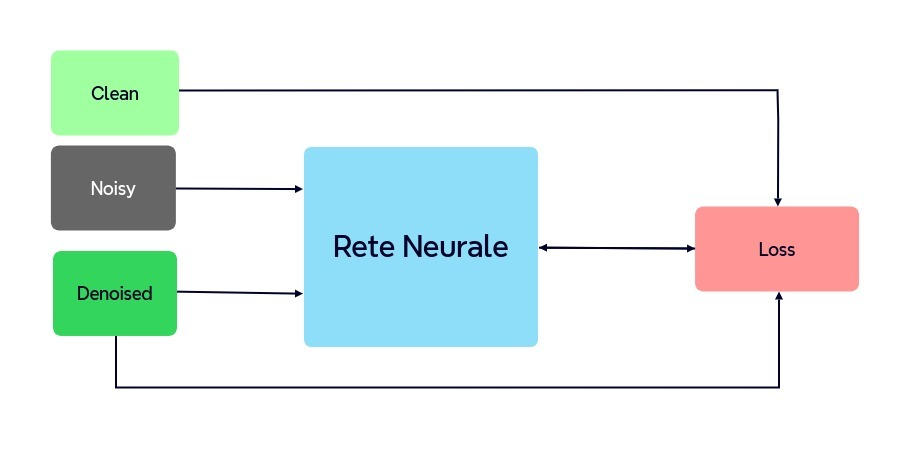
\includegraphics[width=0.8\textwidth]{utils/Architettura_rete_neurale.jpg}
    \caption{Mock della struttura della rete neurale per la previsione della qualità}
    \label{fig:MockReteNeurale}
\end{figure}

Come illustrato in Figura \ref{fig:MockReteNeurale}, il dataset impiegato è costituito da tre tipologie di 
immagini: clean, noisy e denoised. Queste immagini sono state realizzate tramite uno strumento ottico di un
satellite per poi essere sporcate con speckle artificiale e su cui infine è stato fatto denoising. Questa scelte è stata fatta
in quanto risulta difficile reperire un dataset contenente immagini SAR abbastanza grande per poter 
addestrare una rete neurale. Le immagini su cui viene fatto l'addestramento sono relative ad un singolo modello di despeckling ed ad 
un determinato look. Quest'ultimo è una metrica che indica l'intensità dello speckle artificiale, in quanto a più look 
corrispondono più catture di quella che è la realtà di interessa e quindi si ha una maggior precisione e uno speckle ridotto.
In fase di addestramento, le immagini noisy e denoised vengono concatenate in un unico tensore a due canali e utilizzate come 
input per la rete neurale. Le immagini clean, invece, assieme a quelle denoised, vengono impiegate per la 
generazione della mappa di qualità, che costituisce il riferimento necessario per 
il calcolo della funzione di perdita. Questo permette al modello di imparare a 
prevedere la qualità del denoising relative ad un dato modello di despeckling e ad determinato   
% !TEX root = ../Thesis.tex

\chapter{Numerical results}

This is where you show that the novel `thing' you described in Chapter~\ref{cap:proposal} is, indeed, much better than the existing versions of the same.

You will probably use figures (try to use a high-resolution version), graphs, tables, and so on. An example is shown in Figure~\ref{fig:dave}.

\begin{figure}[htbp]
\begin{center}
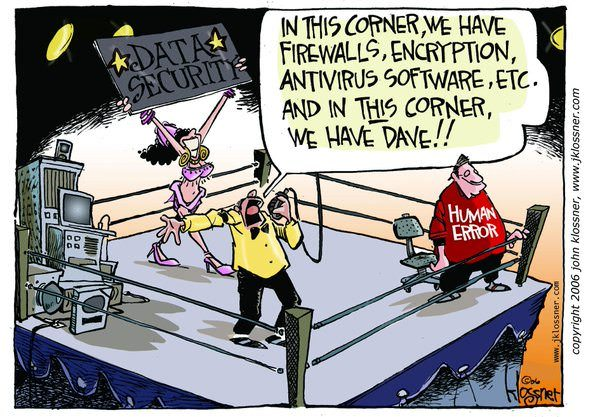
\includegraphics[width=.7\textwidth]{DaveSecurity}
\caption{Network Security - the sad truth}
\label{fig:dave}
\end{center}
\end{figure}

Note that, likewise tables and listings, you shall not worry about where the figures are placed. Moreover, you should not add the file extension (LaTeX will pick the `best' one for you) or the figure path.

% !TEX root = ../Thesis.tex

\chapter{Conclusions and Future work}

They say that the conclusions are the shortened version of the introduction, and while the Introduction uses future verbs (we will), the conclusions use the past verbs (we did). It is basically true.

In the conclusions, you might also mention the shortcomings of the present work and outline what are the likely, necessary, extension of it.
E.g., we did analyse the performance of this network assuming that all the users are pedestrians, but it would be interesting to include in the study also the ones using bicycles or skateboards.

Finally, you are strongly encouraged to carefully spell check your text, also using automatic tools (like, e.g., Grammarly\footnote{\url{https://www.grammarly.com/}} for English language).

%--------------------------------------------------------------
% Bibliography
%--------------------------------------------------------------
\bibliographystyle{plain} 
\bibliography{Bibliography} % Entries are in the Bibliography.bib file

%--------------------------------------------------------------
\end{document}
%--------------------------------------------------------------
